\section{Hardware Platform}
\label{sec:back:hw}

This project targets the EFM32GG microcontroller by Silicon Labaratories.
The following sections describes the various options supplied by SiliconLabs and the platform used in the work leeding up to this thesis.

\subsection{EFM32}
The EFM32GG is a versatile chip aimed at low power application with support for number of peripherals.
The chip called Giant Gecko by SiliconLabs is a part of their energy friend range of 32-bit microcontrollers.
\autoref{tab:efm32-family} shows that the Giant Gecko lies in the upper end of this range.

\begin{table}[H]
  \centering
  \begin{tabular}{|l|l|l|l|l|}
    \hline
    Family & Core & Speed (MHz) & Flash Memory (kB) & RAM (kB) \\
    \hline
    Zero Gecko & ARM Cortex-M0+ & 24 & 4, 8, 16, 32 & 2, 4 \\
    Tiny Gecko & ARM Cortex-M3 & 32 & 4, 8, 16, 32 & 2, 4 \\
    Gecko & ARM Cortex-M3 & 32 & 16, 32, 64, 128 & 8, 16 \\
    Leopard Gecko & ARM Cortex-M3 & 48 & 64, 128, 256 & 32 \\
    Giant Gecko & ARM Cortex-M3 & 48 & 512, 1024 & 128 \\
    Wonder Gecko & ARM Cortex-M4 & 48 & 64, 128, 256 & 32 \\
    \hline
  \end{tabular}
  \caption{EFM32 Product Family \cite{web:silabs}}
  \label{tab:efm32-family}
\end{table}

\subsection{Evaluation boards}

SiliconLabs provides a range of Boards and Kits for development and testing purposes.

For development and testing purposes, SiliconLabs provides two hardware kits with the Gecko.
The simplest of the two are the Giant Gecko Starter Kit depicted in \autoref{fig:efm32gg-stk3700}.
This board contains a few leds, buttons, sensors, a segment LCD display and an expansion header.

\begin{figure}[H]
  \begin{center}
    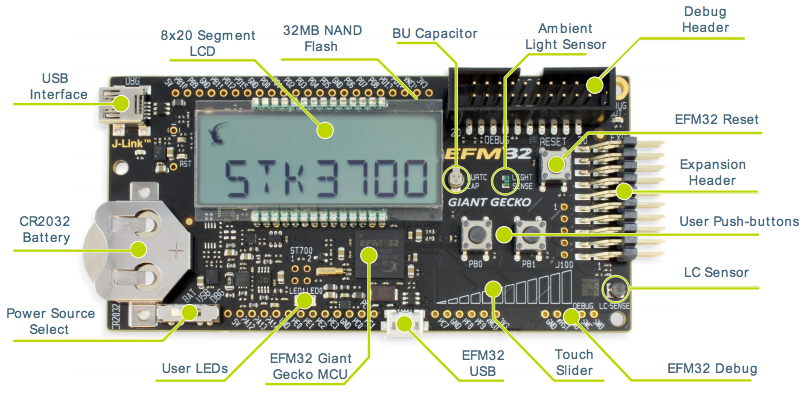
\includegraphics[scale=0.4]{figures/efm32gg-stk3700}
  \end{center}
  \caption{The Giant Gecko Starter Kit - EFM32GG-STK3700 \cite{UM-STK} }
  \label{fig:efm32gg-stk3700}
\end{figure}

As seen in \autoref{fig:efm32gg-dk3750} the Giant Gecko Development Kit is a more complex board.
It features a touch TFT Display, a prototyping board and a plugable MCU board containing the Gecko.

\begin{figure}[H]
  \begin{center}
    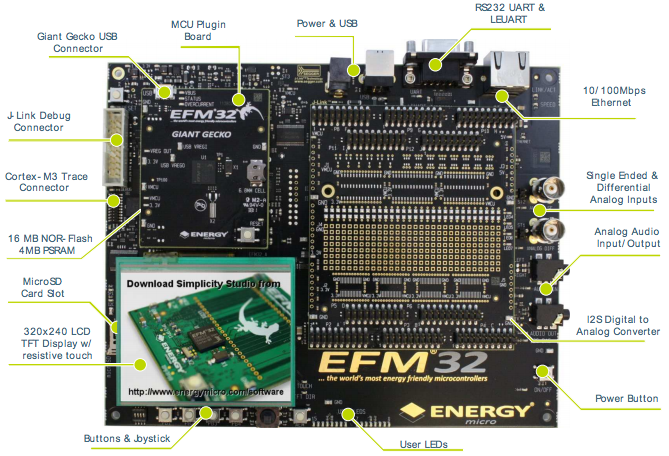
\includegraphics[scale=0.5]{figures/efm32gg-dk3750}
  \end{center}
  \caption{The Giant Gecko Development Kit - EFM32GG-DK3750 \cite{UM-DK}}
  \label{fig:efm32gg-dk3750}
\end{figure}

Table \ref{tab:hw:boards} summarizes the different hardware devices refered to throughout this thesis.

\begin{table}[H]
  \begin{tabular}{|c|c|c|}
    \hline
    Product Name & Description & Short name \\
    \hline
    \hline
    EFM32GG & The Giant Gecko Microcontroller & Gecko \\
    \hline
    EFM32GG-STK3700 & Giant Gecko Starter Kit & STK \\
    \hline
    EFM32GG-DK3750 & Giant Gecko Development Kit & DK \\
    \hline
    BIOMETRIC-EXP-EVB & Biometric Sensor Expansion Board & BIO-EXP \\
    \hline
  \end{tabular}
  \caption{Hardware devices}
  \label{tab:hw:boards}
\end{table}

In addition to the two board mentioned above, the Biometrix-EXP Evaluation board is used for additional sensors.
The BIO-EXP in \autoref{fig:biometric-exp} connects to the STK Expansion Header.

\begin{figure}[H]
  \begin{center}
    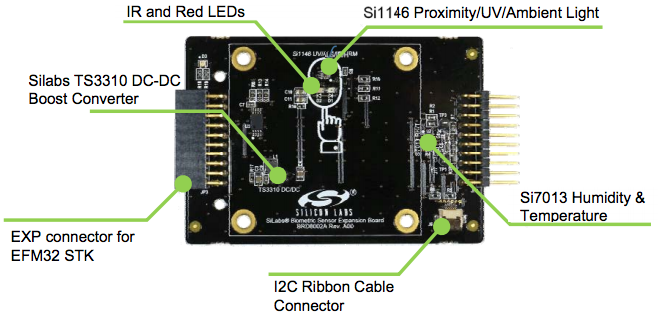
\includegraphics[scale=0.5]{figures/biometric-exp}
  \end{center}
  \caption{The Biometric-EXP Evaluation Board - BIOMETRIC-EXP-EVB \cite{UG-BIO-EXP}}
  \label{fig:biometric-exp}
\end{figure}
